\documentclass[]{standalone}
\usepackage{amsmath}
\usepackage{amssymb}
% No page numbers and no paragraph indentation                                  
\pagestyle{empty}                                                               
\setlength{\parindent}{0bp}%
\usepackage{graphicx}
\usepackage{tikz}
\usepackage{xcolor}
\usetikzlibrary{calc,fadings,decorations.pathreplacing,shapes,shapes.multipart,arrows,shapes.misc,intersections,positioning}

\begin{document}

\tikzset{
    partial ellipse/.style args={#1:#2:#3}{
        insert path={+ (#1:#3) arc (#1:#2:#3)}
    }
}

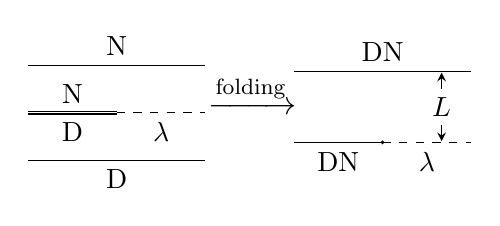
\begin{tikzpicture}[scale = 0.75]
\draw (0,0.2) -- ++(3,0);
\draw (0,1.8) -- ++(3,0);
\draw (0,1.02) --++( 1.5, 0);
\draw (0,0.98) --++( 1.5, 0);
\node[above] () at (1.5,1.8) {N};
\node[below] () at (1.5,0.2) {D};
\node[above] () at (0.75,1) {N};
\node[below] () at (0.75,1) {D};
\node[below] () at (2.25,1) {$\lambda$};
\draw[dashed] (1.5,1) --++( 1.5, 0);
\node[above] () at (3.8,0.8) {\large $\xrightarrow{\rm folding}$};
\begin{scope}[shift={(4.5,0.5)}]
\draw (0,0) -- (1.5,0);
\draw[dashed] (1.5,0) -- (3,0);
\draw[fill] (1.5,0) circle (0.02);
\draw (0,1.2) -- (3,1.2);
\draw[-stealth] (2.5,0.9)--(2.5, 1.18);
\draw[-stealth] (2.5,0.3)--(2.5, 0.02);
\node () at (2.5,0.6) {$L$};
\node[below] () at (0.75,0) {DN};
\node[below] () at (2.25,0) {$\lambda$};
\node[above] () at (1.5,1.2) {DN};
\end{scope}
\end{tikzpicture}


\end{document}